% !Mode:: "TeX:UTF-8"
%%% Local Variables:
%%% mode: latex
%%% TeX-master: t
%%% End:

%实体属性和关系路径知识库补全

\chapter{结合关系路径和实体属性的知识库补全}
\label{cha:kbc-lit-relation}

\section{问题引入}
大规模的知识库包含大量的实体、关系和属性值,并使用三元组的形式对现实世界中实体关系等各种知识进行表示,知识库中的三元组包括实体关系型和实体属性型两大类。实体关系型三元组形如(北京师范大学,位于,北京),其中“北京师范大学”和“北京”分别表示关系型三元组的头实体和尾实体,“位于”表示是关系路径特征;实体属性型三元组形如(北京师范大学,建校于,1902年),其中 “北京师范大学”是头实体,“建校于”是实体属性特征,“1902年”是具体的实体属性特征值。
虽然许多知识库的规模很大,但他们仍然是不完备的,如很多人的出生地点并未包含在知识库中,一些演员是否出演过某些电影也是未知的。为了解决这个问题,很多知识库补全的方法被提出来,这类方法的基于知识库中已有的三元组预测新的三元组,如提供一些三元组(北京师范大学,位于,北京)、(北京师范大学,有校长,董奇)、(董奇,居住在,北京)、(北京,位于,中国),我们希望能构建一种关系机器学习模型,预测(北京师范大学,位于,北京)这个三元组是否正确。
传统的基于关系路径的知识库补全算法通过抽取实体对之间的关系路径进行关系预测,本部分的研究主要研究如何结合大量的关系路径特征和实体属性特征进行知识库补全的模型预测。

\begin{figure}[H]
\begin{center}
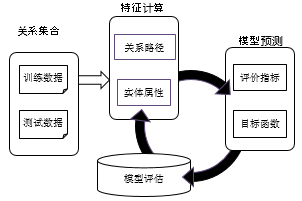
\includegraphics [width=0.5\textwidth]{frame1.PNG}
\caption{知识库补全计算框架}
\label{frame}
\end{center}
\end{figure}

本研究提供一种结合关系路径特征和实体属性特征的知识库补全方法。
通过提取知识库中实体的关系路径特征和实体属性特征,构建模型,进行知识库的实体关系预测。
除此之外,本论文研究了基于学习排序算法进行知识库补全的技术,在传统基于分类器模型的基础上,
提出了非线性的排序算法,对知识库候选实体对进行排序计算,获得更优的候选实体对排序集合。

图\ref{frame}展示了本部分基于逻辑符号的知识库补全算法基本框架。其中对于每个关系集合,将集合切分为训练集和测试集。
模型的训练分为两个部分:(1)特征计算,包括关系路径特征计算和实体属性特征计算两个部分;(2)模型预测,包括基于分类模型的逻辑回归算法,基于树模型的学习排序算法,基于深度神经网络的排序算法等。根据对模型预测评价指标的不同,不断调整预测模型参数,
使得模型能够达到最优的结果。

\section{结合实体属性和关系路径特征}
特征计算是知识库补全的特征抽取阶段,特征的数量和特征有效性是决定知识库补全效果的关键点之一。
给定一个完整的知识库,我们将知识库中的实体和关系分别转化为图中的顶点和边,
这样就能构建一个基于图模型的知识库补全系统。对于知识库中每种待预测的关系,
我们抽取对应关系下的实体对,将实体对的头实体和尾实体在图中进行随机游走\cite{Lao2012},
获得连接头实体和尾实体的关系路径特征,从而获得了知识库补全的关系路径特征。
给定一个目标关系r和这个关系对应的实体对集合
$$I_s=\{(s_j,t_j)|<s_j,t_j> \in KB\}$$

我们期望找出连接头尾实体对的关系路径特征。
由于连接头尾实体对之间的路径数量很大,通常需要限定关系路径的长度,
并采用随机游走算法计算选择从头实体到尾实体的关系路径,将这些路径集合作为关系路径特征。
对于能连接从头实体到尾实体的关系路径,我们记录这个关系路径的类型,作为模型预测的特征。
我们计算0-1二值化后的的路径类型,作为关系路径特征的特征值。对于每个关系抽取的关系特征,我们最终记为$V_r$ $(h_i,t_i)$作为关系路径特征,表示从头实体到尾实体有哪些关系路径进行连接。
例如对于实体对(北京师范大学,位于,北京)三元组,我们可以基于上述的关系路径抽取算法获得
(北京师范大学,位于,北京市海淀区,位于,北京)、(北京师范大学,有校长,董奇,居住在,北京)等多条路径来
获得关系“位于”对应的关系路径类型特征。

本论文通过枚举不同维度的实体属性特征,计算这些实体对在这些实体属性特征下的特征值。
属性特征抽取过程较为复杂,不仅需要考虑不同类型的属性信息不一致问题,也要研究如何处理缺失值问题。
首先对于每个实体,有着不同类型的描述特征,如一个人的信息,不仅有出生年月这种时间类型的信息,
也有年龄、性别等不同种类的属性信息。我们采用了对实体信息进行标准化的方法,
将实体对的头实体和尾实体这些不同属性特征进行归一化处理范围限定在[0,1]之间。
进行归一化后计算获得新的属性特征记为$V_l(h_i)$和$V_l (t_i)$,分别表示头实体和尾实体在所有熟悉特征下的实体属性特征向量,其中$h_i$ 和$t_i$表示给定关系l的第i个头实体和尾实体,同时我们对于头实体和尾实体进行相减计算获得$V_l(h_i-t_i )$属性值。除此之外,对于很多实体在不同特征上的缺失值,我们将缺失值进行了补0处理,期望获得更优结果。
如对于“北京师范大学”这个实体,我们抽取了他的“建校时间”、“占地面积”等所有的实体属性特征,
并计算每个实体对在这些特征下标准化、归一化等特征工程转化后的特征值,而且将缺失属性特征补0。
除了抽取不同类型的关系路径和实体属性特征,构建实体对的特征向量,如何能更好结合实体属性特征和关系路径特征也是知识库补全的重要研究问题之一。

\section{关系路径特征计算}
\label{sec:relational-compute}
特征计算是知识库补全的特征抽取阶段,特征的数量和特征有效性是决定知识库补全效果的关键点之一。
给定一个完整的知识库,我们将知识库中的实体和关系分别看做为图中的顶点和边,
这样就能构建一个基于图模型的知识库补全系统。对于知识库中每种特定待预测的关系,
我们抽取对应关系下的实体对,将实体对的头实体和尾实体在图中进行随机游走\cite{Lao2012},
获得连接头实体和尾实体的关系路径特征,从而获得了知识库补全的关系路径特征。
给定一个目标关系r和这个关系对应的实体对集合
$$I_s=\{(s_j,t_j)|<s_j,t_j> \in KB\}$$


\subsection{关系路径类型集合}
\label{sec:relational-set}
我们期望找出给定关系下,所有连接头尾实体对的关系路径特征,最终获得一个关系路径类型的集合。
在知识库中,由于连接头尾实体对之间的路径数量很大,通常需要限定关系路径的长度,一般限定图中的关系路径长度在2-6之间。

对于能连接从头实体到尾实体的关系路径,我们记录这个关系路径的类型,作为模型预测的特征。
我们采用随机游走算法\cite{Lovsz1993RandomWO}计算选择从头实体到尾实体的关系路径,将这些路径集合作为关系路径类型特征集合。
例如对于实体对(北京师范大学,位于,北京)三元组,我们可以基于上述的关系路径抽取算法获得
(北京师范大学,位于,海淀区,位于,北京)、(北京师范大学,有校长,董奇,居住在,北京)等多条路径来
获得关系“位于”对应的关系路径特征。对于上述两条关系路径,我们抽取关系路径中的关系类型,
生成一个关系路径类型集合,包括(位于 -位于)和(有校长-居住在)
等不同关系组成的关系路径类型,从将多种不同的关系路径类型结合而构成一个关系路径类型集合。对于反方向的关系路径我们采用
${relation}^{-1}$表示。

\subsection{关系路径特征向量}
获取关系路径类型集合(记为S(r))后,我们将给定关系r下的实体对$(s_j,t_j)$计算所有关系路径类型集合下的特征值。
如果实体对$(s_j,t_j)$在集合S(r)中的某个关系路径$s_i$存在,则我们可以将该实体对的对应关系路径类型的特征值记为1,
否则该实体对在这个关系路径类型下的特征值记为0,这种算法简化了不同关系类型在知识库中的权重,但是一些实验表明\cite{Gardner2014}
进行0-1二值化可以简化关系路径类型特征和特征值计算过程,同时对于实验结果的影响并不显著。为了能在不影响模型效果的前提下,
加速我们的计算过程,我们对自己的关系路径类型特征值计算进行了0-1二值化。

\section{实体属性特征计算}
\label{sec:literal-compute}
除了\ref{sec:relational-compute}中计算得到的关系路径类型,考虑到在知识库中任然存在大量的实体属性特征并未被使用,
本研究也对每个关系下的实体属性特征进行计算,获得这些实体属性特征下的特征值。
实体属性特征获取较为简单,只需要枚举知识库中存在的不同实体属性类型,即可这些实体属性类型作为实体特征集合。
实体属性特征的处理和计算是获取更有效特征、提升知识库补全算法的关键。

属性特征抽取过程较为复杂,不仅需要考虑不同维度的属性信息不一致问题,也要研究如何处理缺失值问题。
本论文通过枚举不同维度的实体属性特征,计算这些实体对在这些实体属性特征下的特征值。
首先对于每个实体,有着不同类型的描述特征,如一个人的信息,不仅有出生年月这种时间类型的信息,
也有年龄、性别等不同种类的属性信息。我们采用了对实体信息进行标准化的方法,
将实体对的头实体和尾实体这些不同属性特征进行归一化处理范围限定在[0,1]之间。
进行标准化后计算获得新的属性特征记为$V_l(h_i)$和$V_l (t_i)$,分别表示头实体和尾实体在所有熟悉特征下的实体属性特征向量,其中$h_i$ 和$t_i$表示给定关系l的第i个头实体和尾实体,同时我们对于头实体和尾实体进行相减计算获得$V_l(h_i-t_i )$属性值。除此之外,对于很多实体在不同特征上的缺失值,我们将缺失值进行了补0处理,期望获得更优结果。
如对于“北京师范大学”这个实体,我们抽取了他的“建校时间”、“占地面积”等所有的实体属性特征,
并计算每个实体对在这些特征下标准化后的特征值,而且将缺失属性特征补0。

在对每个关系下的实体对集合进行实体属性特征抽取计算后,我们获得了这个关系下头实体的实体属性特征、尾实体的实体属性特征、
对头尾实体进行归一化后的归一化实体属性特征,以及头实体和尾实体差值计算得到的实体属性特征。

通过将\ref{sec:relational-compute}关系路径特征和\ref{sec:literal-compute}抽取的实体属性特征进行结合,构建结合实体属性特征和关系路径特征的组合特征,从而获得了由关系路径特征、头实体属性特征、尾实体属性特征、头尾实体结合属性特征、结合关系路径类型和实体属性类型特征组合的特征向量,从而获得每个关系下所有实体对组合构建的特征矩阵,并构建机器学习模型对生成的特征矩阵进行学习预测,获得知识库补全中的实体对的关系。


\section{关系路径和实体属性特征实验}

本研究通过抽取关系路径特征和实体属性特征,并对抽取特征进行正则化特征工程后,构建了基于逻辑回归的预测模型,期望能进行研究分析,发掘如何更好结合关系路径和实体属性特征的方法。如图\ref{literal-relation-compute}所示,我们获取知识库中的关系型特征类型即关系路径特征类型和非关系型特征类型即实体属性特征类型,将两种特征相互融合构建实体对的预测向量,从而构建预测模型进行知识库补全模型训练,获得每个关系下的知识库补全训练模型,从而能更好进行知识库补全预测。

\begin{figure}[H]
\begin{center}
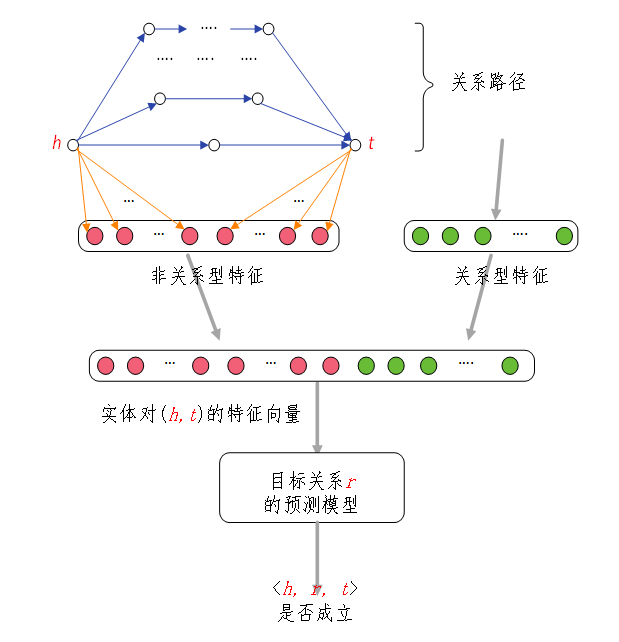
\includegraphics [width=0.7\textwidth]{literal-relation-compute.PNG}
\caption{结合实体属性和关系路径知识库补全计算过程}
\label{literal-relation-compute}
\end{center}
\end{figure}

本研究的实验分为两组,包括基于YAGO知识库和基于Freebase知识库的模型预测评估。尽管有很多大规模的知识库,但考虑到这些知识库需要包含关系三元组和实体属性三元组,我们选择了这些知识库实体和关系丰富的YAGO2和Freebase知识库,并选择了YAGO和Freebase中实体属性丰富的实体关系组成集合,构建组成YAGO和FB15K数据集。对于这些知识库中的实体关系,我们抽取其中实体属性特征较多的三元组,作为一个训练预测数据,从而避免很多缺少实体属性三元组的实体在实体关系缺失时影响模型效果。

表\ref{tab:addlabel-kbcExp-data}中展示了YAGO和Freebase知识库的基本数据情况。我们选择了YAGO和Freebase中具有较多属性特征的实体关系三元组,并通过PRA、SFE算法抽取这些三元组的关系路径特征,同时,我们从知识库中抽取每个实体的实体属性特征类型,并计算这些实体属性特征值,将两者结合组成预测实体关系的特征向量。本章节的实验中我们选择三元组的正负实体对比例是1:4,选择YAGO和Freebase中实体的要求是,每个实体在知识库中有超过5个及以上的实体属性值。

% Table generated by Excel2LaTeX from sheet 'Sheet2'
\begin{table}[htbp]
  \centering
  \caption{知识库基本数据统计}
    \begin{tabular}{|l|r|r|}
    \hline
    \textcolor[rgb]{ .141,  .161,  .18}{} & \multicolumn{1}{l|}{FB15K} & \multicolumn{1}{l|}{YAGO} \\
    \hline
    实体    & 14951 & 58130 \\
    \hline
    关系类型  & 1345  & 32 \\
    \hline
    实体属性类型 & 336   & 25 \\
    \hline
    属性三元组 & 25776 & 141606 \\
    \hline
    关系三元组 & 592213 & 499350 \\
    \hline
    训练集   & 483142 & 399480 \\
    \hline
    测试集   & 59071 & 49132 \\
    \hline
    \end{tabular}%
  \label{tab:addlabel-kbcExp-data}%
\end{table}%

知识库补全模型采用MAP、MRR、AUC和hit@1多种不同的评估指标进行模型评价,其中MAP、MRR和hit@1是在排序算法中常见的模型评价指标,很多常见知识库补全算法如PRA、SFE和TransE等模型都采用这些指标进行模型评价。AUC是常见的分类和排序模型评价指标,可以很好的衡量二分类时模型预测的效果。这些指标也在各种常见知识库补全、信息检索、图链接预测任务作为评价函数。本研究全面深入的研究了结合实体属性和关系路径的知识库补全算法,为了能全面深入分析不同类型特征带来的模型效果影响,本部分实验使用了上述四种评价指标同时进行模型评估,期望采用客观公正的评价指标,分析我们的算法是否能有效地提高模型效果。

\subsection{YAGO知识库实验}
\label{cha:exp-literal}
本部分的效果展示了在YAGO知识库下进行知识库补全算法的结果,我们的方法和对比方法被分为三类。
其中,SFE-literal(图中简称SFE-lit)和PRA-literal(图中简称PRA-lit)是结合关系路径特征和实体属性特征的方法,SFE-literal是基于子图特征抽取算法(SFE)抽取关系路径特征,并结合literal属性特征构建的特征向量,而PRA-literal是基于路径排序算法(PRA)抽取关系路径特征,并结合literal属性特征构建的特征向量模型。SFE和PRA是只基于关系路径特征进行知识库补全的两种算法,TransE和TransR是基于表示学习中进行知识库补全算法中典型的两种模型,通过学习特征的低维度向量表示,进行知识库中实体和实体之间的关系预测。本部分分析了表示学习算法中知识库补全算法,只基于关系路径的知识库补全算法,结合实体属性和关系路径的知识库补全算法的模型效果。

分析发现,结合literal属性特征的模型,MAP、MRR和AUC预测结果最好,
总体的预测结果稳定,效果好。而仅仅基于关系路径特征,未加实体属性特征的PRA和SFE算法特征较好,
使用表示学习的TransE和TransR模型效果在MAP中预测较差,
但是通过AUC和hit@1进行模型的二分类效果结果和基于符号逻辑的效果相似。
结果显示,加入实体属性特征后,结合实体属性特征和关系路径特征的补全技术,相比只采用关系路径特征的补全技术有更高的准确性,在进行排序相关的预测效果评测时,有较好的效果。
在采用二分类模型进行评价时候,无论是符号逻辑的路径排序相关算法还是表示学习的低维嵌入算法,都能有效的进行模型预测。

从图\ref{tab:kbc-yago-literal}分析三类不同知识库补全算法的四种评估指标可以发现。
相比只采用关系路径的知识库补全算法,结合实体属性特征和关系路径特征的知识库补全算法,
在YAGO数据集合上,MAP预测结果有较大的提升,相比原来的模型,SFE-literal和PRA-literal在计算MAP时,都获得了近1\%的效果提升,模型提升效果统计显著。而传统的基于表示学习的知识库补全算法,
由于进行了低维表示模型近似,无论是MAP还是MRR等各种指标都较基于关系路径的知识库补全算法差别较大。但基于二分类模型评价函数AUC指标进行分析时可以发现,基于关系路径、结合实体关系路径特征和基于表示学习的知识库补全算法,在模型效果上没有显著差异。

基于表\ref{tab:kbc-yago-literal}分析YAGO知识库补全实验可以获得如下结论:(1)预测知识库中新三元组通过结合关系路径特征和实体属性特征能更加的精确有效,无论是以分类为优化目标的分类模型,还是以排序为优化目标的排序问题。
(2)由于在YAGO知识库集合中,有更多的属性事实进行关系预测,采用特征组合,能获得更多的不同类型组合特征,达到更好的优化结果,因此,结合属性事实和关系事实进行预测是非常重要的。
(3)对于某些特殊的关系,进行标准化处理是非常有效的,但是并非对于所有的属性事实进行标准化有效,选择合适的属性特征和实体关系特征进行组合是十分必要的。
(4)本研究的实验结果表明,对于多数YAGO2中的关系来说,我们的属性事实不仅可以用来预测关系事实,
而且还能调整原来的关系特征的路径权重,使得模型预测更加合理。
因此,结合属性事实和更丰富的关系特征能获得更好的知识库补全结果。
% Table generated by Excel2LaTeX from sheet 'yago'
% yago literal result
\begin{table}[htbp]
  \centering
  \caption{YAGO知识库实体属性和关系路径特征模型预测结果}
    \begin{tabular}{|l|r|r|r|r|}
    \hline
          & \multicolumn{1}{l|}{MAP} & \multicolumn{1}{l|}{MRR} & \multicolumn{1}{l|}{AUC} & \multicolumn{1}{l|}{hit@1} \\
    \hline
    SFE-lit & 78.610\% & 100.000\% & 92.994\% & 45.328\% \\
    \hline
    PRA-lit & 78.170\% & 97.830\% & 93.496\% & 45.104\% \\
    \hline
    PRA   & 77.610\% & 97.830\% & 93.258\% & 45.509\% \\
    \hline
    SFE   & 77.360\% & 97.830\% & 93.225\% & 45.502\% \\
    \hline
    transE & 56.400\% & 91.200\% & 92.740\% & 45.642\% \\
    \hline
    transR & 46.470\% & 65.410\% & 92.986\% & 46.128\% \\
    \hline
    \end{tabular}%
  \label{tab:kbc-yago-literal}%
\end{table}%


我们进一步分析了每个关系下关系路径和实体属性特征的权重和特征变化情况,表\ref{tab:lit-rel-kbc}显示了在YAGO知识库中的集种关系典型:Export、GraduateFrom、HasAcademicAdvisor,通过结合实体属性特征和关系路径特征,学习获得的重要权重。相比于路径排序算法这种只使用关系特征进行预测的方式,
结合属性事实特征不仅仅能增加模型预测的全面性具有更好的模型泛化能力,还能将模型预测结果精度提高,同时也能调整逻辑回归算法中不同关系路径特征和不同属性事实特征的权重,对于部分不重要的特征起到特征选择的作用。通过将关系路径特征和属性事实特征进行结合,使得模型的预测结果更加可靠。
如表所示,我们分析关系“graduateFrom”可以发现,除了常见的关系路径特征:
isCitizenOf $\to$ isCitizenOf$^{-1}$ $\to$ livesIn $\to$ isLocatedIn$^{-1}$、
isAffiliatedTo$^{-1}$ $\to$ isCitizenOf $\to$ livesIn $\to$ isLocatedIn$^{-1}$
等,部分关系路径特征重要性发生变化,部分关系路径特征在模型训练中被特征选择筛出,从而获得了新的更具有预测能力的关系路径特征。同时我们也可以发现一些重要的实体属性特征如:wasCreatedOnDate、happenedOnDate等都在关系预测结果中有着重要的作用。通过分析这些关系路径特征、实体属性特征的权重我们可以发现,实体属性特征不仅能提高关系预测中的精度,有较高的准确性,同时也能调整关系路径的权重,产生更多的有表达力的关系路径特征。这表明进行知识库补全模型预测的时候,结合关系路径和实体属性特征能有效进行组合从而获得更具有模型泛化能力的特征向量。

\begin{table}[htbp]
  \centering
  \caption{YAGO知识库关系路径和实体属性特征比较}
    \begin{tabular}{cp{10.3cm}|p{3.7cm}|}
    \hline
    \multicolumn{3}{c}{Export} \\
    \hline
    \multirow{5}[2]{*}{PRA} & imports$\to$ hasMusicalRole$^{-1}$$\to$ hasMusicalRole &  \\
          & livesIn$^{-1}$$\to$ diedIn$\to$ imports  &  \\
          & livesIn$^{-1}$$\to$ wasBornIn$\to$ dealsWith$^{-1}$ $\to$ imports &  \\
          & isCitizenOf$^{-1}$$\to$ influences$^{-1}$ $\to$ isCitizenOf$^{-1}$ $\to$ imports &  \\
          & isCitizenOf$^{-1}$$\to$ wasBornIn $\to$ dealsWith$^{-1}$ $\to$ imports &  \\
    \hline
    \multirow{5}[2]{*}{PRA-lit} & hasCapital $\to$ hasCapital$^{-1}$ $\to$ exports & hasGini \\
          & imports $\to$ hasMusicalRole$^{-1}$ $\to$ hasMusicalRole$^{-1}$ & hasInfaltion \\
          & isCitizenOf$^{-1}$ $\to$ wasBornIn $\to$ hasCapital$^{-1}$ $\to$ exports & hasEconomicGrowth \\
          & exports $\to$ hasMusicalRole$^{-1}$ $\to$ hasMusicalRole & hasPoverty \\
          & isInterestedIn$^{-1}$$\to$ wasBornIn $\to$ hasCapital$^{-1}$ $\to$ exports& wasDestroyedOnDate \\
    \hline
    \multicolumn{3}{c}{GraduateFrom} \\
    \hline
    \multirow{5}[2]{*}{PRA} & isCitizenOf $\to$ isCitizenOf$^{-1}$ $\to$ livesIn $\to$ isLocatedIn$^{-1}$&  \\
          & diedIn $\to$ happenedIn$^{-1}$ $\to$ participatedIn$^{-1}$ $\to$ isLocatedIn$^{-1}$ &  \\
          & hasWebsite $\to$ hasWebsite$^{-1}$ $\to$ livesIn $\to$ isLocatedin$^{-1}$ &  \\
          & isAffiliatedTo $\to$ isAffiliatedTo$^{-1}$ $\to$ isCitizenOf $\to$ isLocatedIn$^{-1}$ &  \\
          & isAffiliatedTo$^{-1}$ $\to$ isCitizenOf $\to$ livesIn $\to$ isLocatedIn$^{-1}$ &  \\
    \hline
    \multirow{5}[2]{*}{PRA-lit} & isAffiliatedTo $\to$ isAffiliatedTo$^{-1}$ $\to$ isCitizenOf $\to$ isLocatedIn$^{-1}$& happenedOnDate\\
          & hasAcademicAdvisor $\to$ hasAcademicAdvisor$^{-1}$ $\to$ graduatedFrom &wasDestroyedOnDate \\
          & hasWebsite $\to$ hasWebsite$^{-1}$ $\to$ livesIn $\to$ isLocatedin$^{-1}$ & wasDestroyedOnDate\\
          & isAffiliatedTo $\to$ isAffiliatedTo$^{-1}$ $\to$ isLeaderOf $\to$ isLocatedIn$^{-1}$ & wasCreatedOnDate \\
          & isCitizenOf $\to$ isCitizenOf$^{-1}$ $\to$ livesIn $\to$ isLocatedIn$^{-1}$ & wasBornOnDate \\
    \hline
    \multicolumn{3}{c}{HasAcademicAdvisor} \\
    \hline
    \multirow{5}[2]{*}{PRA} & wasBornIn $\to$ happenedIn$^{-1}$ $\to$ participatedIn$^{-1}$ $\to$ livesIn$^{-1}$ &  \\
          & diedIn $\to$ hasCapital$^{-1}$ $\to$ isLocatedIn$^{-1}$ $\to$ diedIn$^{-1}$ &  \\
          & worksAt $\to$ graduatedFrom$^{-1}$ $\to$ livesIn $\to$ wasBornIn$^{-1}$ &  \\
          & hasAcademicAdvisor $\to$ hasAcademicAdvisor$^{-1}$$\to$ influences$^{-1}$ $\to$ hasAcademicAdvisor &  \\
          & livesIn$\to$ diedIn $\to$ hasAcademicAdvisor &  \\
    \hline
    \multirow{5}[2]{*}{PRA-lit} & hasGender $\to$ hasGender$^{-1}$ & wasDestroyedOnDate \\
          & worksAt $\to$ graduatedFrom$^{-1}$ $\to$ livesIn $\to$ wasBornIn$^{-1}$ & hasHeight \\
          & hasAcademicAdvisor $\to$ hasAcademicAdvisor$^{-1}$ $\to$ diedIn $\to$ diedIn$^{-1}$ & hasHeight \\
          & diedIn $\to$ diedIn$^{-1}$ $\to$ livesIn $\to$ livesIn$^{-1}$ & wasBornOnDate \\
          & graduatedFrom $\to$ worksAt $\to$ worksAt$^{-1}$ $\to$ worksAt  & diedOnDate \\
    \hline
    \hline
    \end{tabular}%
  \label{tab:lit-rel-kbc}%
\end{table}%
% Table generated by Excel2LaTeX from sheet '工作表1'


\subsection{Freebase知识库实验}

% fb15k实验结果
\begin{table}[htbp]
  \centering
  \caption{Freebase知识库实体属性和关系路径特征模型预测结果}
    \begin{tabular}{|l|r|r|r|r|}
    \hline
          & \multicolumn{1}{l|}{MAP} & \multicolumn{1}{l|}{MRR} & \multicolumn{1}{l|}{AUC} & \multicolumn{1}{l|}{hit@1} \\
    \hline
    transR & 66.440\% & 95.500\% & 86.182\% & 44.145\% \\
    \hline
    transE & 72.910\% & 98.650\% & 89.118\% & 47.348\% \\
    \hline
    SFE   & 86.490\% & 98.650\% & 97.087\% & 55.559\% \\
    \hline
    SFE-lit & 86.560\% & 100.000\% & 97.140\% & 55.636\% \\
    \hline
    PRA   & 86.930\% & 98.200\% & 97.021\% & 55.527\% \\
    \hline
    PRA-lit & 87.140\% & 100.000\% & 97.108\% & 55.606\% \\
    \hline
    \end{tabular}%
  \label{tab:addlabel-fb}%
\end{table}%
本部分的效果展示了在Freebase知识库下进行知识库补全算法的结果,我们的方法和对比方法也被分为三类:结合关系路径和实体属性的知识库补全、基于关系路径的知识库补全和基于表示学习的知识库补全算法,每组实验中都选择两种典型的算法进行实验分析。和YAGO知识库补全实验相似,表\ref{tab:addlabel-fb}展示了在不同评价指标下Freebase知识库中部分关系的预测结果。
其中,SFE-literal和PRA-literal是结合关系路径特征和实体属性特征的方法,PRA和SFE是只基于关系路径特征的知识库补全算法,TransE和TransR是基于表示学习、低维向量的知识库补全方法。其中结合实体属性和关系路径特征的知识库补全模型评价的MAP、MRR和AUC预测结果最好,
尤其在采用AUC进行模型评价时候,相比于表示学习方法,基于符号逻辑的知识库补全算法特征有非常高的提升。从基于MAP和MRR的评价指标来看,加入实体属性特征的总体预测结果最稳定,效果最好,而未加实体属性特征的PRA和SFE特征较好,
使用表示学习的TransE和TransR模型效果在MAP中预测较差,
结果显示,加入实体属性特征后,结合实体属性特征和关系路径特征的补全技术,相比只采用关系路径特征的补全技术有更高的准确性,在进行排序相关的预测效果评测时,有较好的效果。
在采用二分类模型进行评价时候,无论是符号逻辑的路径排序相关算法还是表示学习的低维嵌入算法,都能有效的进行模型预测。

总体上看,使用MAP、MRR、AUC以及hit@1评价指标时,基于符号逻辑的知识库补全算法效果较基于表示学习的算法性能有较大的提升,而结合实体属性特征和结合关系路径特征的知识库补全算法相比仅仅使用关系路径特征的模型效果更好。这说明无论采用分类作为模型的优化方向,还是采用实体对排序的序列作为知识库补全优化目标,使用符号逻辑相比于近似的表示学习方法效果都有明显的提升。


分关系来看,从表\ref{tab:addlabel-fb-map}中分析Freebase中的各个关系预测结果的MAP值。
我们可以发现,在Freebase的15种关键关系中,
我们通过采用结合关系路径特征和实体属性特征的知识库补全算法,相比于只采用关系路径的知识库补全算法,我们的模型效果在MAP排序指标上有很大的提升。如/tv/tv/genreprograms、/film/actor/film/film/performance/film和 /film/director/film 、/media/commonnetflix/genretitles等关系使用MAP评测都有较大的模型效果提升。

% Table generated by Excel2LaTeX from sheet 'FB15K'
\begin{table}[htbp]
  \centering
  \caption{FB15K部分关系MAP得分}
    \begin{tabular}{|p{5.8cm}|p{1.4cm}|p{1.4cm}|p{1.4cm}|p{1.4cm}|p{1.4cm}|p{1.4cm}|} %{|l|r|r|r|r|r|r|}
    \hline
    MAP-score & \multicolumn{1}{l|}{PRA-lit  } & \multicolumn{1}{l|}{PRA} & \multicolumn{1}{l|}{SFE-lit} & \multicolumn{1}{l|}{SFE} & \multicolumn{1}{l|}{transE} & \multicolumn{1}{l|}{transR} \\
    \hline
    /people/person/profession & 12.150\% & 11.902\% & 12.359\% & 12.096\% & 77.134\% & 71.784\% \\
    \hline
    /film/actor/film/film/performance/film & 28.309\% & 26.179\% & 22.121\% & 20.560\% & 87.007\% & 78.431\% \\
    \hline
    /media/common/netflix/genre/titles & 50.135\% & 48.281\% & 49.919\% & 49.546\% & 63.788\% & 65.603\% \\
    \hline
    /people/ethnicity/people & 57.143\% & 57.143\% & 57.143\% & 57.143\% & 60.402\% & 50.396\% \\
    \hline
    /film/film/genre/films/in/this/genre & 57.285\% & 55.650\% & 41.435\% & 41.828\% & 68.762\% & 64.254\% \\
    \hline
    /music/instrument/instrumentalists & 58.268\% & 58.268\% & 58.268\% & 58.268\% & 53.702\% & 52.452\% \\
    \hline
    /music/genre/artists & 69.514\% & 69.514\% & 69.514\% & 69.514\% & 77.745\% & 65.328\% \\
    \hline
    /location/location/time/zones & 77.479\% & 77.130\% & 77.479\% & 77.479\% & 82.790\% & 72.245\% \\
    \hline
    /tv/tv/genre/programs & 80.952\% & 80.952\% & 80.952\% & 80.952\% & 78.140\% & 60.484\% \\
    \hline
    /people/person/nationality & 81.119\% & 79.616\% & 81.774\% & 80.770\% & 75.448\% & 73.757\% \\
    \hline
    /people/cause/of/death/people & 82.653\% & 82.653\% & 82.653\% & 82.653\% & 52.979\% & 44.508\% \\
    \hline
    /music/record/label/artist & 83.704\% & 83.704\% & 83.704\% & 83.704\% & 55.037\% & 41.867\% \\
    \hline
    /film/production/company/films & 85.561\% & 85.561\% & 85.561\% & 85.561\% & 68.758\% & 59.189\% \\
    \hline
    /film/director/film & 100.000\% & 100.000\% & 100.000\% & 100.000\% & 94.077\% & 88.385\% \\
    \hline
    /film/film/directed/by & 100.000\% & 100.000\% & 100.000\% & 100.000\% & 95.254\% & 85.679\% \\
    \hline
    \end{tabular}%
  \label{tab:addlabel-fb-map}%
\end{table}%

我们以关系/people/person/nationality和关系/film/actor/film/film/performance/film进行分析,研究关系路径特征和实体属性特征在路径排序算法中的特征表现。通过分析MAP指标来看,TransE和TransR这两个模型在各个关系上的效果较为稳定,符号逻辑相关算法在这些不同的关系上效果差别较大,通过分析相关的关系路径和实体属性权重,我们可以发现,这些关系路径特征相对于YAGO知识库来说,关系路径权重区别并不明显,甚至在结合实体属性特征后,对于/film/actor/film/film/performance/film这个关系来说,所有的关系路径和实体属性路径特征综合从44120减少到42787种特征。
说明基于随机游走抽取的关系路径特征并不能很好的区分Freebase中实体和实体之间的关系,
但是当加入关系路径特征后,能很好的惩罚这些加入区分度不好的关系路径特征。

其次尽管部分关系相对于表示学习来说,预测结果的效果较差,但是,基于图模型的知识库补全系统中,大部分关系的预测相对于基于表示学习效果提升很多。这一方面说明基于表示学习是一种近似的模型预测,而基于符号逻辑的关系路径学习排序则是一种精确而有效的学习方式。另一方面也说明,
在知识库构建的图模型中,部分关系较为稀疏的实体之间使用表示学习,预测结果较为理想,
而采用结合实体属性和关系路径的符号逻辑补全算法,则能基于有效的关系路径,获得十分有用的预测模型结果。

其次,由于Freebase知识库总共包含超过1345种不同类型的关系,这些关系覆盖了电影、人种、电视剧、音乐等不同类型的关系,这些不同的关系中部分关系具有对称性,一些关系和关系之间差别很大,
如何能将这些不同类型互不影响或者相互对称的关系区分出来,构建一个合理的图,基于这种合理的图模型进行关系路径的抽取和实体属性特征的计算,是未来研究的重要研究步骤。

\section{本章工作总结}
本部分通过抽取了实体属性类型、关系路径类型作为知识库补全的特征向量类型,并通过计算每个关系下实体对的实体属性特征值和关系路径特征值。将这些特征值进行组合,并构建了简单的逻辑回归算法模型,通过再不同知识库中的实验,评估了不同类型特征组合的情况下,我们结合关系路径特征和实体属性特征相比传统的关系路径特征计算问题,在分类预测、排序预测评估指标下的优势。

在接下来的章节中,本研究将通过构建不同的机器学习模型,比较逻辑回归分类算法、基于学习排序的树模型、深度学习模型等来评估知识库补全算法应该如何选择预测模型。 